\subsection{Introduction to the Mobile Network}
In 2010, it was estimated that the total global mobile phone subscriber base 
exceeded 3.8 billion users \citep{mpirical10}. These figures can be categorised 
into the following geographical areas, as show in figure \ref{fig:subscriberBase} 
below.

\begin{figure}[H]
  \centering
    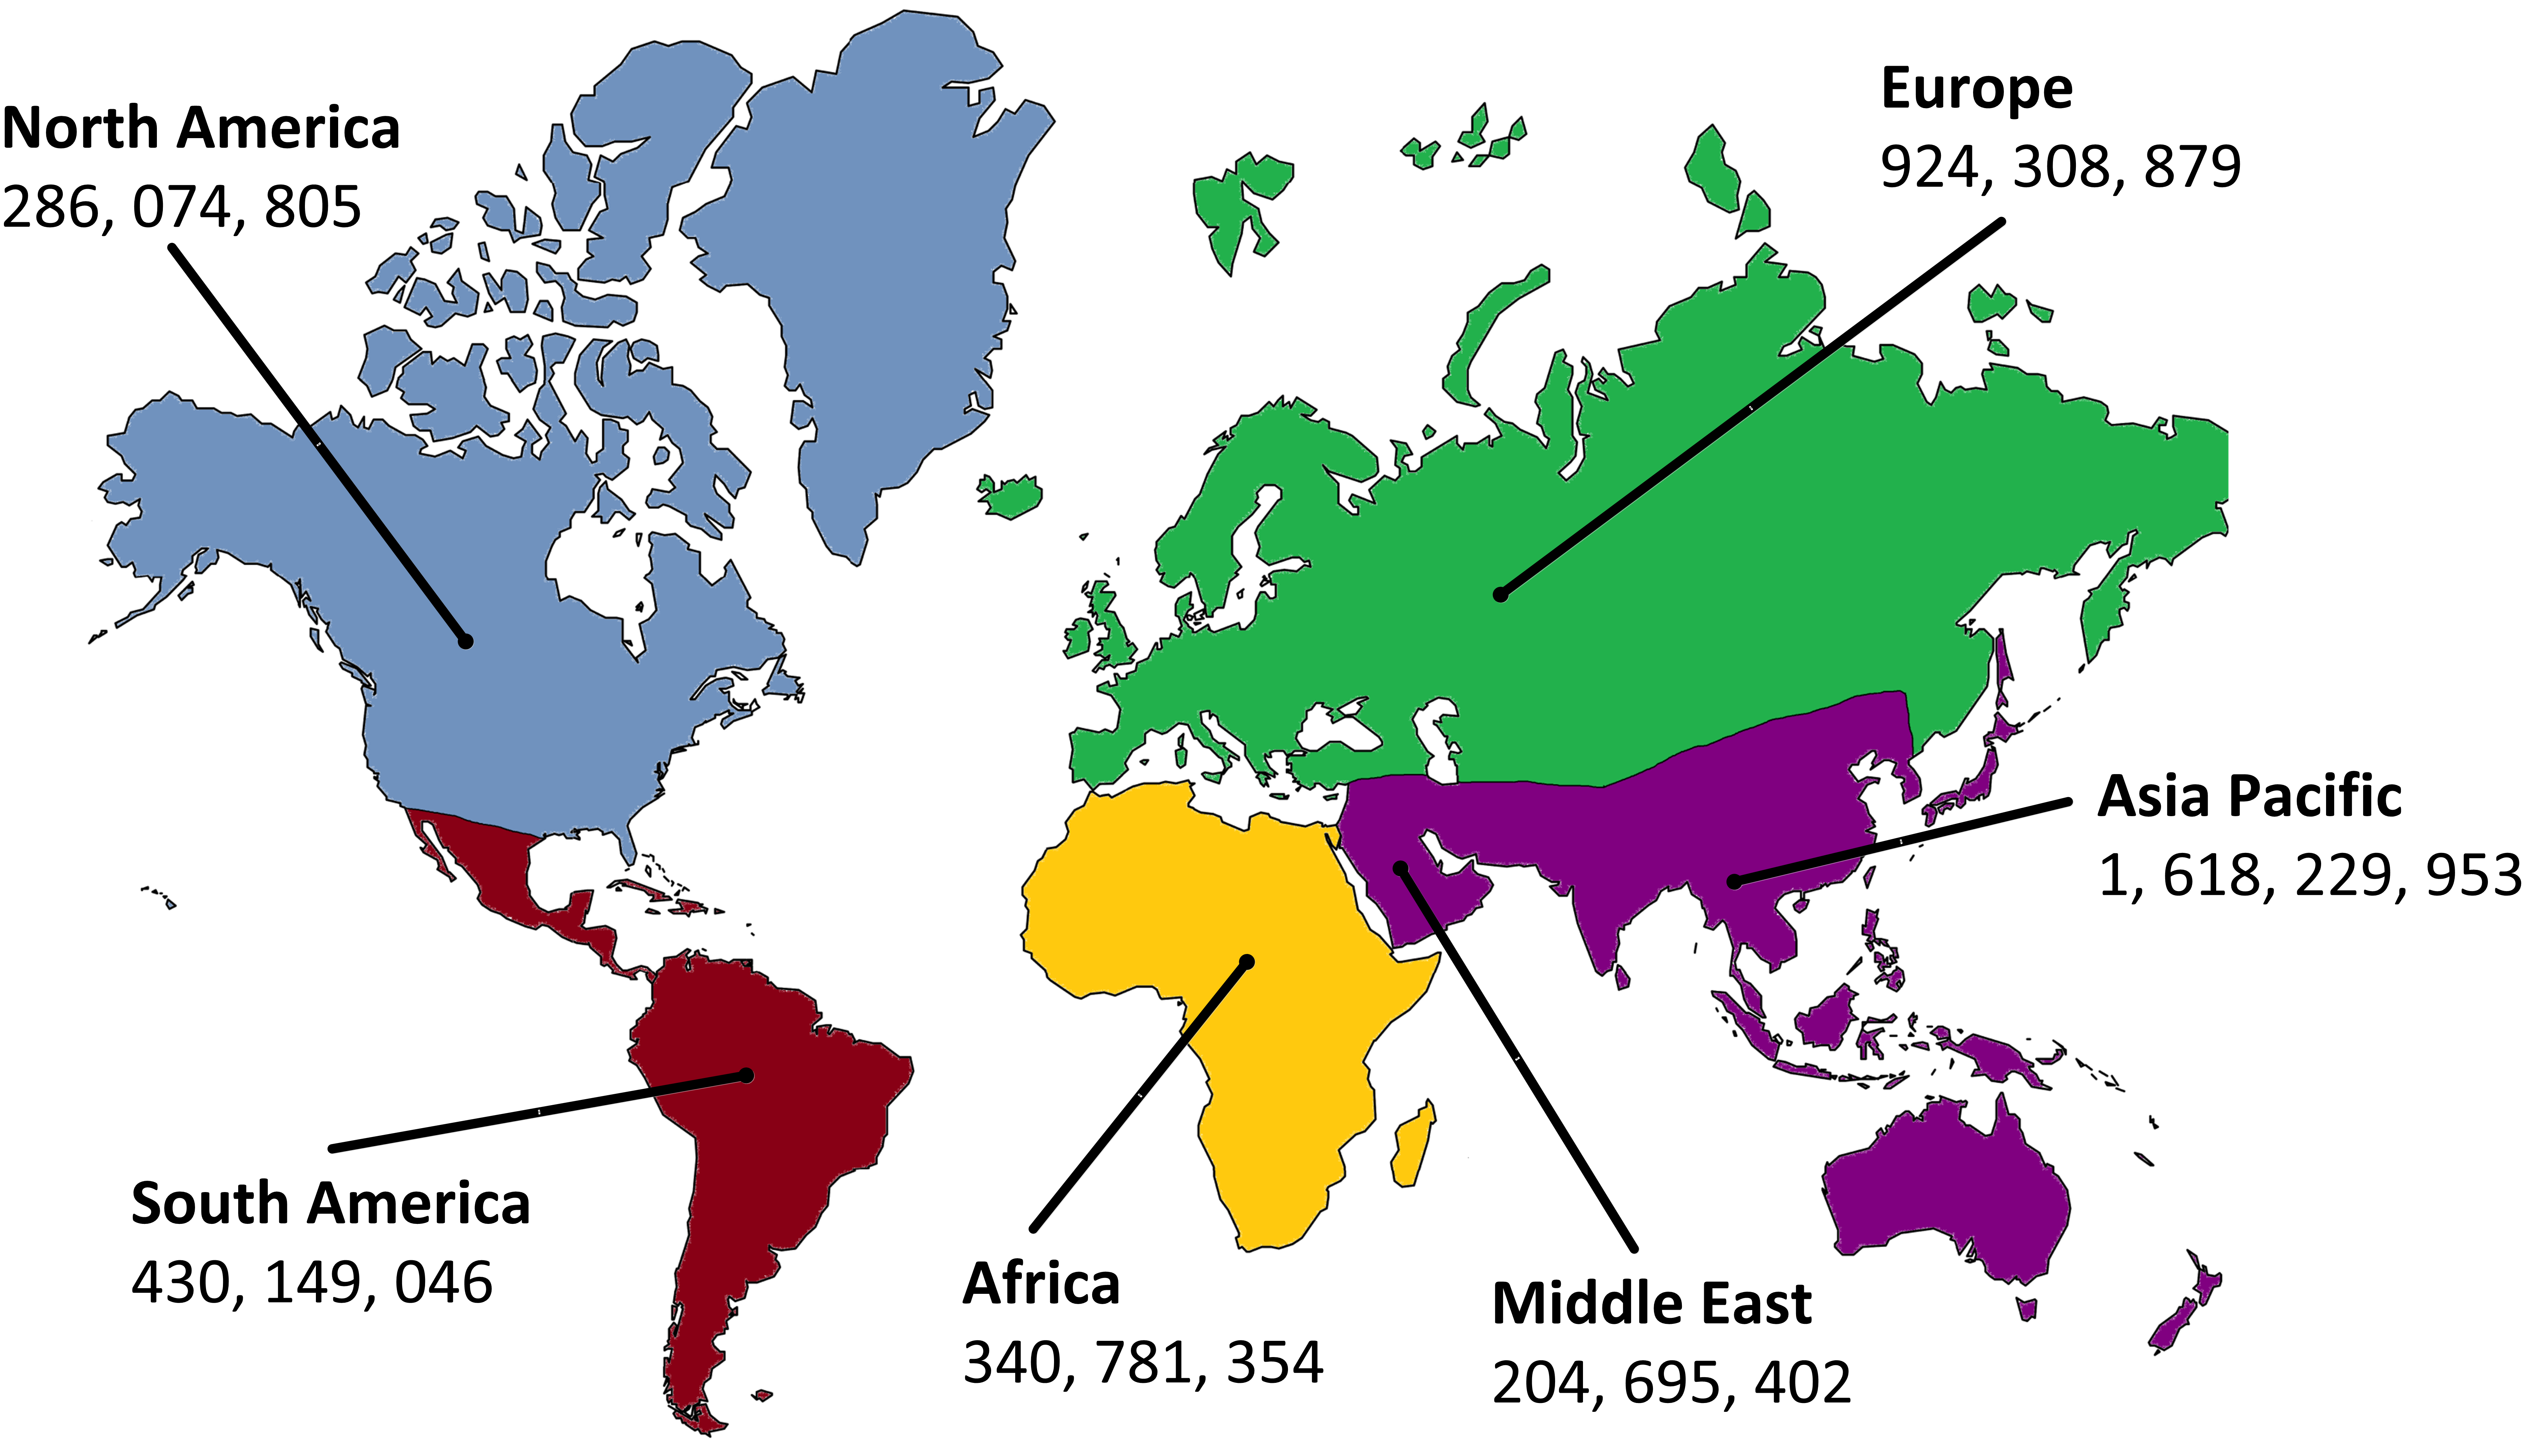
\includegraphics[width=0.8\textwidth]{chapter3/mobile_networks/subscriber_numbers.png}
  \caption{An indicator of the physical size of each region.}
  \label{fig:subscriberBase}
\end{figure}


Since the original mobile phone was first introduced in the 1980s, the 
underlying technology had gone through four major phases, known as generations 
\citep{cox08}.

The first generation of mobile phones (1G) utilised analogue communication 
techniques. These devices were famously bulky and expensive, and during the 
mid-1990s the second generation (2G) was introduction \citep{cox08}.

The second generation utilised the more powerful digital communication 
techniques, which allowed for the cost of the technology to reduce rapidly and 
for more services to be run. These additional services are now widely use and 
examples are text messaging, email and basic internet access \citep{cox08}.

Third generation (3G) and the newer fourth generation (4G) phones still utilise 
the digital communications spectrum. However the phones send and receive their 
signals in a different way from their predecessors, and from each other 
\citep{cox08}. 

For example 4G devices utilises a two antenna system, whereas the 3G only 
utilises one. The result of this is that the devices are able to support higher
data rates, which allows for video calls and high speed internet access.

A cellular system will be controlled by a particular operator (e.g. EE, O2 or 
Vodafone) and is referred to as a public land mobile network (PLMN). The PLMN 
has three aspects \citep{cox08}:
\begin{itemize}
  \item The Core Network
  \item The Radio Access Network
  \item The Mobile Phone
\end{itemize}

This is visualised within figure \ref{fig:mobileSystem} below.

\begin{figure}[H]
  \centering
    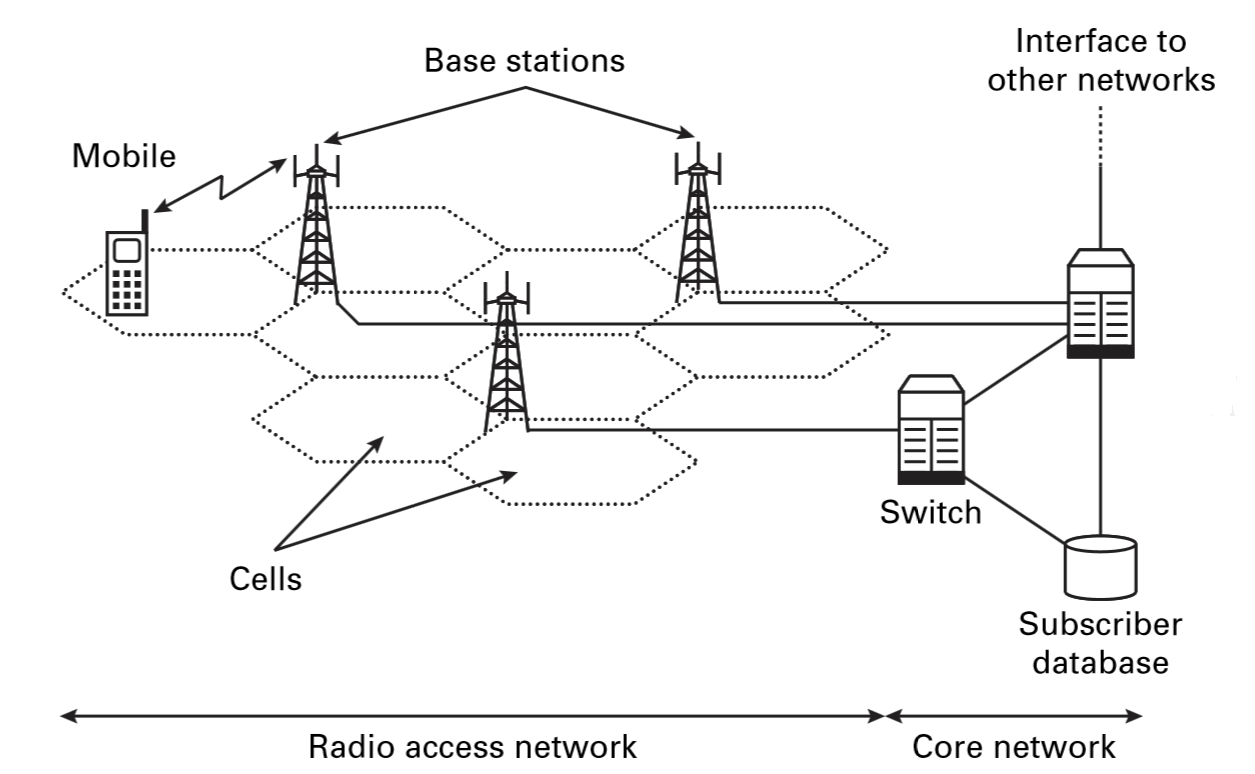
\includegraphics[width=0.8\textwidth]{chapter3/mobile_networks/mobile_architecture.png}
  \caption{The basic concept behind the mobile telecommunication system.}
    \label{fig:mobileSystem}
\end{figure}

The core network mimics a traditional fixed line telephone network. It's 
objective is to send voice calls or text messages from one phone to another 
using various switches. These switches could be thought as network switches 
found in computer networks \citep{cox08}.

The core network will also maintain a database containing information about the
network operator’s subscribers, as well as monitoring the locations of mobile 
phones. Monitoring each mobile phone's location, allows for an always-on style 
of connection to the mobile network, hence allowing calls to be made upon the
move \citep{cox08}.

The radio access network (RAN) ``handles the radio communications between the 
core network and the mobile phone'' \citep{cox08}. It contains a large number 
of base stations, each of which transmits and receives radio signals to and 
from the mobile phones in the surrounding area.

Each base station is equipped with multiple directional antennas \citep{cox08}, 
and will support one or more cells –-- usually three \citep{mpirical10}.

Each cell will have a maximum size –-- determinate by the largest distance that 
radio signals can be successfully sent and received \citep{cox08}. A radio wave
that interacts with objects (such as trees, buildings, hills, cars, people etc)
will have a huge impact upon coverage \citep{mpirical10}.

In order to gain the maximum radio coverage, radio planners will utilise various 
modelling and planning tools which are able to predict the likely coverage for 
a given area \citep{mpirical10}.

These tools allow for the minimisation of costs and maximisation of cell 
coverage, by determining the best location for each base station 
\citep{mpirical10}.

Figure \ref{fig:signalStrength} highlights the coverage area for a 2G base 
station. The base station is highlighted by a cross with a circle around it
\citep{mpirical10}.

\begin{figure}[H]
  \centering
    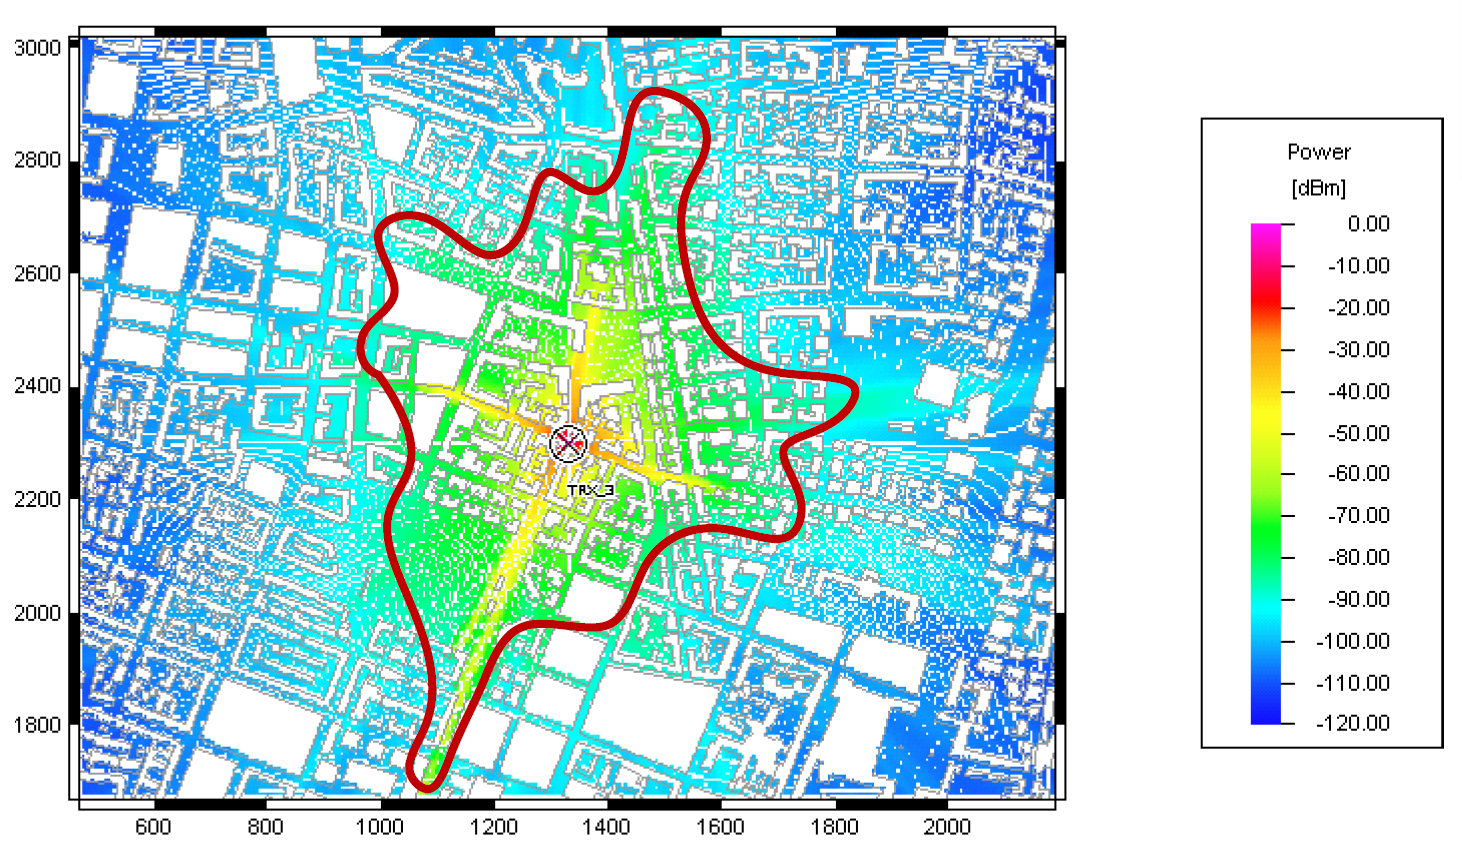
\includegraphics[width=0.8\textwidth]{chapter3/mobile_networks/mobile_network_intensity.png}
  \caption{An example output from a network modelling tool.}
  \label{fig:signalStrength}
\end{figure}

Figure \ref{fig:signalStrength} shows that some areas receive a stronger signal
than others, and as previously mentioned this is related to the number of 
objects within the areas that degrade the signal strength. To counter this 
mobile networks arrange cells upon a hierarchical structure \citep{mpirical10}. 
Each cell can be classified as either a:
\begin{itemize}
  \item Macro Cell
  \item Micro Cell
  \item Pico Cell
\end{itemize}

A Marco Cell is able to provide wide scale coverage. These cells are generally 
found within rural areas in which the usage would be deemed light. The radio 
antenna for a Macro Cell is usually found at the top of radio masks, to ensure 
the largest coverage possible \citep{mpirical10}.

A Micro Cell is able to provide street level coverage. These cells are 
generally found within urban areas and can be used in areas where coverage is 
high. The radio antenna for a Micro Cell is usually found upon the side of 
buildings or upon small street level masks \citep{mpirical10}.

A Pico Cell is able to provide room or building level of coverage. These cells 
are generally found within office or home spaces where the usage is extremely 
high. The radio antenna for a Pico Cell is usually found within one corner of 
a room or within the ceiling \citep{mpirical10}.

Figure \ref{fig:cellHierarchy} outlines the various different types of cells as 
a hierarchical diagram \citep{mpirical10}.

\begin{figure}[H]
  \centering
    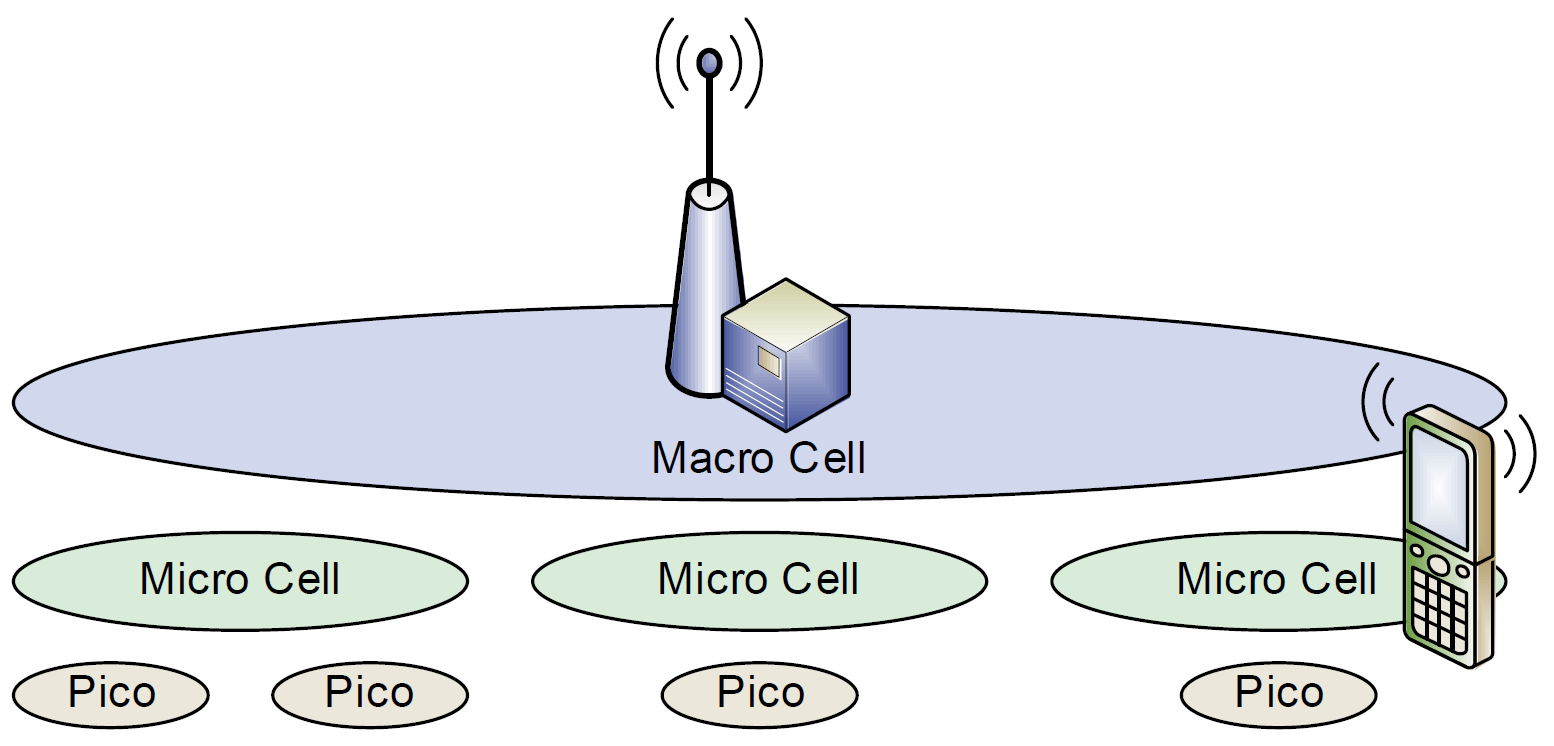
\includegraphics[width=0.80\textwidth]{chapter3/mobile_networks/network_hierarchy.png}
  \caption{Cell hierarchical structure.}.
  \label{fig:cellHierarchy}
\end{figure}

The main reason for using cells within the mobile system is that it allows for 
radio frequencies to be reused in difference locations. The reuse of frequencies 
simply allows for more mobile phones to be supported at any one given time 
\citep{cox08}. This setup also prevents any co-channel interface 
\citep{mpirical10}.

So far the term mobile phone has been used. However due to technological 
changes in recent years, mobile phones are not the only sole device that can 
access the mobile network. For example cellular dongles, tablet computers, 
cameras, e-readers and card readers are just a small number of devices that are 
able to use the cellular network. 

It is for this reason that the term user equipment (UE) is officially used 
within the Universal Mobile Telecommunications System (UMTS) specification 
instead of the term mobile phone \citep{cox08,mpirical10}. 

Throughout this project, the term device and UE will be used interchangeably. 
